\documentclass[11pt, oneside]{article}   	% use "amsart" instead of "article" for AMSLaTeX format
\usepackage{geometry}                		% See geometry.pdf to learn the layout options. There are lots.
\geometry{letterpaper}                   		% ... or a4paper or a5paper or ... 
\usepackage{graphicx}				% Use pdf, png, jpg, or eps§ with pdflatex; use eps in DVI mode
								% TeX will automatically convert eps --> pdf in pdflatex		
\usepackage{amssymb}
\usepackage{mhchem}


\date{}							% Activate to display a given date or no date
\parindent 0in
\parskip 6pt

\begin{document}
 
\section*{Introduction to Box Models}
 
Box models are a simple class of models used to study the behavior of a system.  In Earth Sciences, they are used to understand the exchange of matter between interconnected reservoirs such as lakes, oceans and the atmosphere; matter is transferred between these reservoirs via rivers, currents, rainfall and evaporation. Box models can be used to answer questions about how a system will respond dynamically (i.e., over time)  to perturbations. In other words, how does a system of reservoirs respond in time to varying inputs and outputs? For example, how does the mass in a lake respond to changes in the input and output fluxes from rivers? Or how does the concentration of a toxic pollutant in rainwater runoff impact its concentration in a lake over time?

We will begin with a simple box model consisting of a single reservoir with mass $M$ and input flux $F_{in}$ and output flux $F_{out}$, as shown in Figure \ref{BoxModel1}. The fluxes  $F_{in}$ and $F_{out}$ have units of mass per unit time.  

\begin{figure}[htbp]
\begin{center}
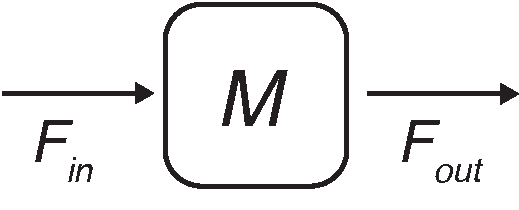
\includegraphics{BoxModel1.pdf}
\caption{A simple box model consisting of a reservoir with mass $M$ and input flux $F_{in}$ and output flux $F_{out}$. }
\label{BoxModel1}
\end{center}
\end{figure}

In this example, the reservoir could represent a lake with total water mass $M$ and the fluxes are from a river flowing in ($F_{in}$)  and a river flowing out ($F_{out}$).  

We can use the principle of {\it conservation of mass}, which states that mass can neither be created nor destroyed (but it can be moved around), to write a simple differential equation:
\begin{eqnarray}
\frac{dM}{dt} = F_{in} - F_{out} \label{dmdt}.
\end{eqnarray}
This equation says that the time rate of change of mass  in the reservoir ($\frac{dM}{dt}$) is equal to the difference between the input and output fluxes. For example, if there is no outlet river then $F_{out}=0$ and the lake will mass will increase  at a rate equal to the input of mass from the input river flux $F_{in}$. Conversely, if there is no input flux $F_{in}=0$, the lake mass will decrease as fast as it is drained by $F_{out}$.  

Let's further consider the   lake-draining example where  $F_{in}=0$. We can integrate the equation to find
\begin{eqnarray}
M(t) = C - F_{out}\, t ,
\end{eqnarray}
where $C$ is an unknown constant.  To find the value of $C$ we must introduce what is referred to as an {\it initial condition}. For our lake example, the initial condition is simply the initial mass of the lake $M_0$ at $t=0$.  Setting $t=0$ in the above equation, we find
\begin{eqnarray}
C = M_0,
\end{eqnarray}
and thus we have
\begin{eqnarray}
M(t) = M_0 - F_{out}\, t.
\end{eqnarray}
You can see that the lake starts with an initial mass and after some time $t$ its mass will be equal to $M_0 - F_{out}\, t$, up until the time when the lake will be completely empty.

A special case of equation \ref{dmdt} is when $F_{in}=F_{out}$. This is known as the {\it steady state} since 
\begin{eqnarray}
\frac{dM}{dt} = 0,
\end{eqnarray}
and the mass of the reservoir is no longer changing.

Now let's consider a more complicated case where the output drainage of the reservoir is proportional to the mass of water in the reservoir, so that $F_{out} = a M$, where $a$ is some positive constant.  This might be more intuitive by thinking about how a river draining a lake will flow faster when the water level of the lake is high (and its mass is larger), whereas during a period of drought  the outlet river flows more slowly due to the lower water level in the lake; in other words the outlet river's flow rate is proportional to the mass in the river.  For the example here we will assume that the inlet river flux is constant, so $F_{in} = b$, where $b$ is some positive constant.  Inserting these into equation \ref{dmdt} gives:
\begin{eqnarray}
\frac{dM}{dt} = b - a M \label{aM}.
\end{eqnarray}
While we are interested in dynamic changes predicted by this equation, its insightful to first consider the steady state solution, which could be reached after a sufficiently long period of time so that $\frac{dM}{dt} = 0$. The state state solution is then
\begin{eqnarray}
\frac{dM}{dt} = 0 = b - a M, \\
M = \frac{b}{a}.
\end{eqnarray}
Thus in the long term, the mass of water in the lake will be equal to the ratio $b/a$ where $b$ is the influx rate and $a$ is the constant of proportionality for the outflux rate. 

Now let's return to the dynamic situation predicted by equation \ref{aM}, which is a relatively simple  ordinary differential equation (ODE).  In this course you will learn how to numerically solve this equation (and much more complicated systems of these equations)  using Python.  Once you learn how to do this in Python, it becomes quite easy to solve increasingly complicated ODE's using a computer.  However, while the numerical solution on a computer is great for its practicality and application to complicated scenarios, it lacks the  insights that can be gained by the symbolic, or mathematical, solution to the ODE. In our example above, the ODE is simple enough that we can solve it using classical integration techniques. 

We begin the analytical solution by rewriting equation \ref{aM} as:
\begin{eqnarray}
\frac{dM}{ b - a M}= dt.
\end{eqnarray}
Integrating both sides of this equation will yield the answer, but the denominator on the left hand side makes it more complicated. We ease this situation by using the substitution $y = b- aM$ which has the differential form $dy = - a\, dM$. Inserting these substitutions and applying the integration gives
\begin{eqnarray}
\int  \frac{dy}{ y} = - a\int dt  = -at + c
\end{eqnarray}
where c is a constant.
The left hand side integral is equivalent to $\ln(y)$, thus we have
\begin{eqnarray}
\int  \frac{dy}{ y} = \ln(y) = -at + c
\end{eqnarray}
\begin{eqnarray}
e^ {\ln(y)} = y =  e^{-at+c} = C\, e^{-at}.
\end{eqnarray} 
Substituting for $y$ and rearranging gives
\begin{eqnarray}
M = \frac{b}{a} - \frac{C}{a} e^{-at}.
\end{eqnarray} 
To get the value of the constant $C$, we  substitute the initial value $M(t=0) = M_0$, giving 
\begin{eqnarray}
C = b - a M_0. 
 \end{eqnarray} 
The resulting equation governing the time evolution of the mass of the lake is then
\begin{eqnarray}
M = \frac{b}{a} - \frac{b - a M_0}{a} e^{-at}.
\end{eqnarray} 
This can be rearranged into a more insightful form:
\begin{eqnarray}
M = \frac{b}{a} (1- e^{-at}) +   M_0 e^{-at}.
\end{eqnarray} 
Think about which terms in this equation dominate when $t=0$. What about when $t$ grows really large?
 
\end{document}  